% Author: Erik Belko <xbelko02@stud.fit.vutbr.cz>

\documentclass[10pt, hyperref={unicode}]{beamer}[3.5.2020]
\usetheme{Dresden}

\usepackage{times}
\usepackage[czech]{babel}
\usepackage[utf8]{inputenc}
\usepackage{graphicx}
\graphicspath{ {img/} }
\usepackage{url}
\usepackage[ruled, czech, linesnumbered, noline, longend]{algorithm2e}
\usepackage{amsthm, amsmath, amssymb}

\usecolortheme{beaver}
\title{Grafové algoritmy}
\author{Erik Belko \texorpdfstring{\\ (xbelko02@stud.fit.vutbr.cz)}{}}
\institute{Vysoké učení technické v~Brne \\ Fakulta informačních technologií}
\date{\today}

\begin{document}

\frame{\titlepage}

\begin{frame}{Přehled}
	\setbeamertemplate{section in toc}[sections numbered]
	\tableofcontents
\end{frame}

\section{Definice grafu}

\begin{frame}{Graf}
    \alert{Graf} (jednoduchý neorientovaný) je uspořádaná dvojice $G = (V, E)$, kde $V$~(verticies) je množina \alert{vrcholů} a~$E$~(edges) je množina \alert{hran}, množina vybraných dvouprvkových množin vrcholů.
    
    \begin{figure}[h]
		\scalebox{0.4}{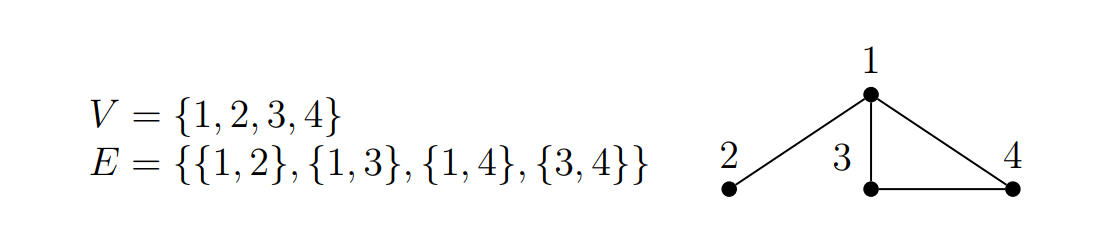
\includegraphics{graf.png}}
    \end{figure}
\end{frame}

\section{Primuv algoritmus}

\begin{frame}{Primův algoritmus}
	\begin{itemize}
		\item<1->
			\alert{Primův algoritmus} (Jarníkův, Primův-Jarníkův nebo i~DJP alg.) je algoritmus hledající minimální kostru souvislého ohodnoceného grafu.
		\item<2->
			Co je to kostra?
			\begin{itemize}
				\item \alert{Kostra grafu} $G$ je jeho podgraf $T$, který je stromem, a~propojuje všechny vrcholy, tedy $V (T) = V (G)$.
			\end{itemize}
		\item<3->
            Najde tedy takovou podmnožinu hran grafu, která tvoří strom obsahující všechny vrcholy původního grafu a~\alert{součet ohodnocení hran} z~této množiny je minimální.
	\end{itemize}
\end{frame}

\subsection{Pseudokód a~Ukázka}

\begin{frame}{Pseudokód}
    Algoritmus začíná s~jedním vrcholem a~postupně přidává další, čímž zvětšuje velikost stromu, dokud neobsahuje všechny vrcholy.
    \IncMargin{1.5em}
        \begin{algorithm}[H]
        \caption{\textsc{Primův algoritmus}}
    	\SetNlSty{}{}{:}
    	\SetInd{-0.25em}{1em}
    	\SetAlgoNlRelativeSize{-1}
    
    	\Indm\Indmm
    	\KwIn{souvislý ohodnocený graf $G (V, E)$}
    	\KwOut{$T(V',E')$ je minimální kostra grafu}
    	\Indp\Indpp
    	\BlankLine
    
    	$V' = \{x\}$, kde $x$ je libovolný vrchol z~$V$, $E' = \{\}$ \\
    	\While{$V' \neq V$} {Vyber hranu $(u,v)$ z~$E$ s~minimální cenou tak, že $u$~patří $V'$ a~$v$~nepatří $V'$
    	\\ Přidej $v$~do $V'$, přidej $(u,v)$ do $E'$}
    	\Return{$T(V',E')$}
        \end{algorithm}
    \DecMargin{1.5em}
\end{frame}

\begin{frame}{Ukázka Primůvho algoritmu}
    \begin{figure}[h]
        \only<1>{\scalebox{0.8}{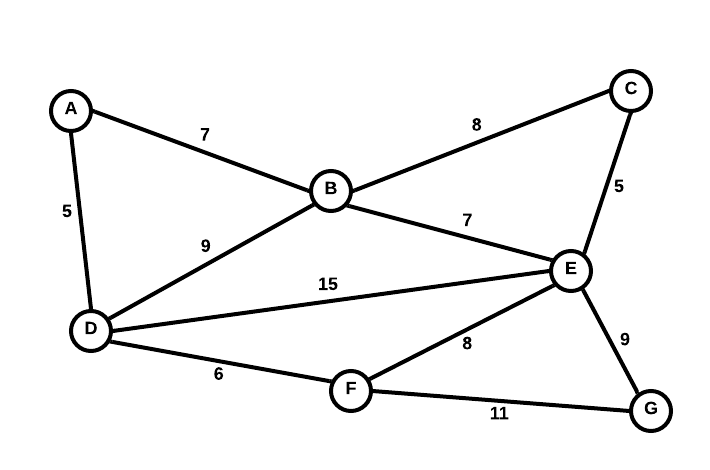
\includegraphics{postup1.png}}}
        \only<2>{\scalebox{0.8}{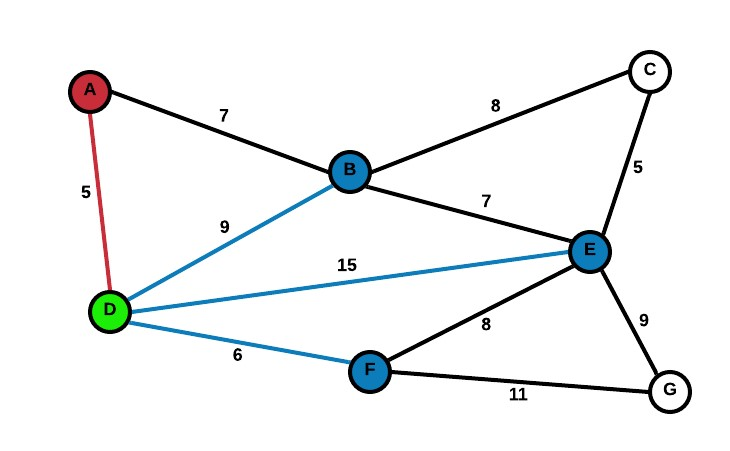
\includegraphics{postup2.jpg}}}
        \only<3>{\scalebox{0.8}{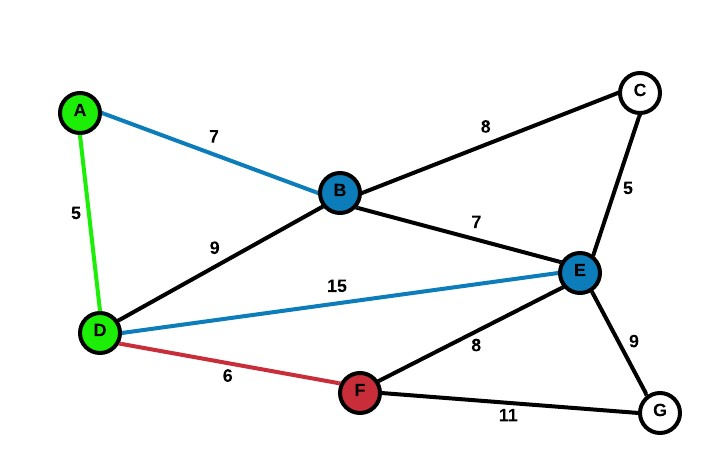
\includegraphics{postup3.jpg}}}
        \only<4>{\scalebox{0.8}{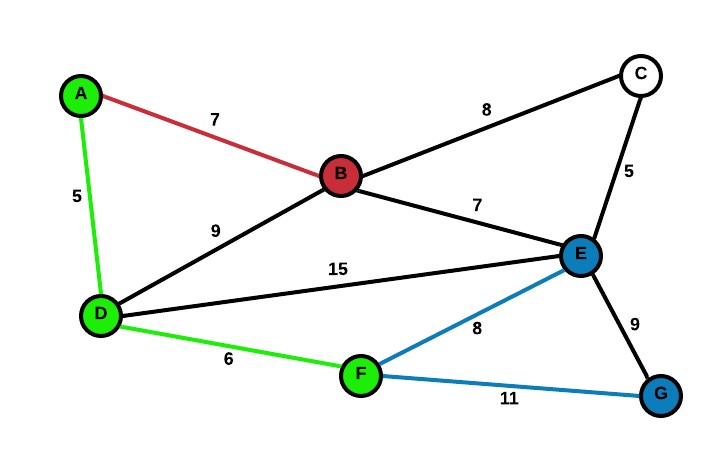
\includegraphics{postup4.jpg}}}
        \only<5>{\scalebox{0.8}{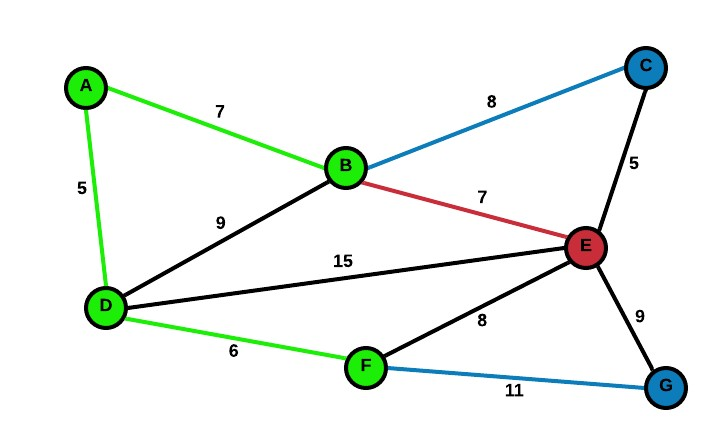
\includegraphics{postup5.jpg}}}
        \only<6>{\scalebox{0.8}{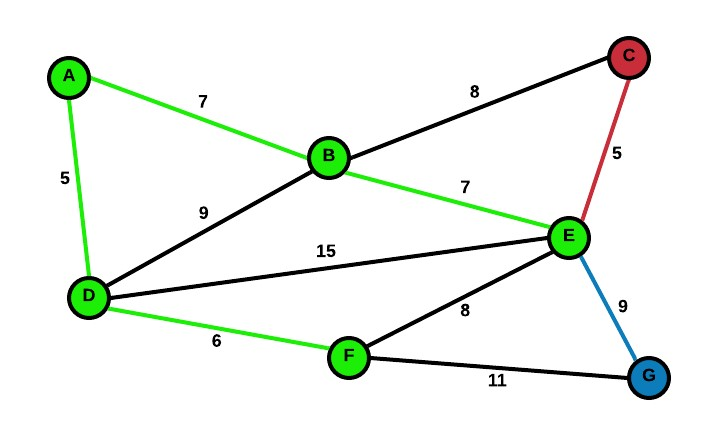
\includegraphics{postup6.jpg}}}
        \only<7>{\scalebox{0.8}{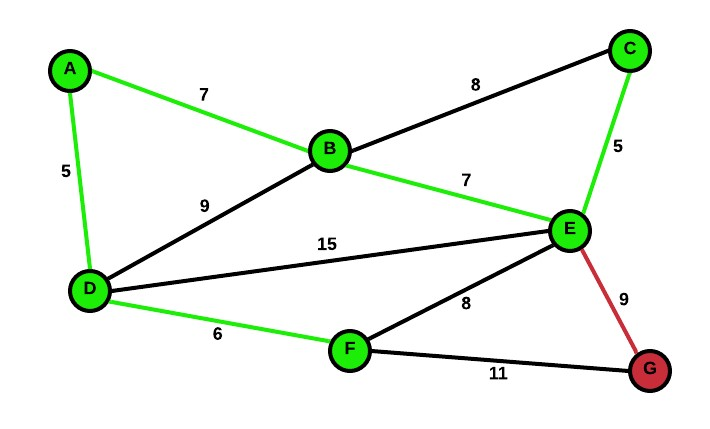
\includegraphics{postup7.jpg}}}
        \only<8>{\scalebox{0.8}{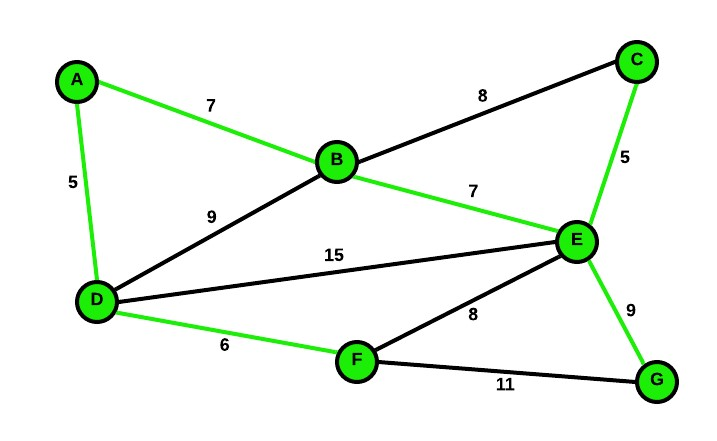
\includegraphics{postup8.jpg}}}
    \end{figure}
\end{frame}

\subsection{Složitost}

\begin{frame}{Složitost}
    \begin{itemize}
        \item Každá hrana má dva konce, proto je testována dvakrát
        \item Potřebný čas je maximálně přímo úměrný $|E| \log_2 |V|$
        \item $|V|$ je počet vrcholů
        \item $|E|$ je počet hran
    \end{itemize}
\end{frame}

\section{Použité zdroje}

\begin{frame}{Použité zdroje}
    \begin{itemize}
        \item Teorie grafů 
        \begin{itemize}
            \item \url{http://www.fit.vutbr.cz/~lengal/idm/grafy-algoritmy.pdf} 
            \item \url{http://www.fit.vutbr.cz/~lengal/idm/grafy-zaklady.pdf}
        \end{itemize}
        \item Primův algoritmus wiki \\ \url{https://sk.wikipedia.org/wiki/Primov_algoritmus}
        \item Primův algoritmus video \\ \url{https://www.youtube.com/watch?v=5pE_0Git5AM}
    \end{itemize}
\end{frame}

\end{document}
